\section{Laboratory work implementation}

\subsection{Frontend}

To create the Frontend of the application i.e. the Views with the UI and the transitions of the views I've followed the steps below:

\begin{itemize}
	\item First thing I've opened the provided PSD files in GIMP as layers and select the layers that I need in my application. Next I've exported the layers as PNG files.
	\item To import them in Android Studio I've used Batch Drawable Importer. It automatically created PNGs for 5 different densities i.e. hdpi, mdpi, xhdpi, xxhdpi and xxxhdpi.
	\item For some parts I needed to encapsulate more images in one object. For this I've created additional drawable file. For example for confirm button I've created a layer-list in the following way : 
	\begin{lstlisting}
<layer-list xmlns:android="http://schemas.android.com/apk/res/android" 
			android:opacity="opaque">
	<!-- The background -->
	<item android:drawable="@drawable/btn__2" />
	
	<!-- The text -->
	<item>
		<bitmap android:src="@drawable/confirm"
				android:gravity="center" />
	</item>
</layer-list>
	\end{lstlisting}
	\item Also I've define the appropriate themes for the app in styles.xml. I have 3 themes:
	\begin{itemize}
		\item TelemedicineTheme - With the background green and with the pattern applied;
		\item TelemedicineTheme.Launch - For the Splash Screen;
		\item TelemedicineThemeMenu - For the views with white background;
	\end{itemize}
	\item At last I've created the layout file for each view I needed;
	\item To make the connection between views and the transitions in each activity class I have the corresponding functions in which I create Intents to start another activity:
	\begin{lstlisting}
	Intent intent = new Intent(this, ClassName.class);
	startActivity(intent);
	\end{lstlisting} 
	\item The functions are called with the help of Click Listeners provided for each button; 
\end{itemize}

\subsection{Backend}

To implement the required functionalities I've used an additional tool i.e. Firebase. Firebase is a web platform which provides developers with tools like Authentication, Database, Hosting etc. to ease the development process for different platforms like Android, IOS, Unity etc.

To bind the application with Firebase services, first we need to create a project in the Firebase console. After creation we can access it. There we have a manager UI from which we can manage the the tools which we are using in the app, e.g. at authentication section we have information about the users, we can manually add them and also the console provides us with nice statistics.  

In what follows I'll enumerate the functionalities:

\begin{itemize}
	\item Authentication/Registration - For Login, Registration and User Storage I've used Authentication tool from Firebase. At the start we also must specify the sign in method. We have different methods e.g. email/password, phone, google etc.
	
	In my classes I'm using a FirebaseAuth(mAuth) and a FirebaseAuth.AuthStateListener(mAuthListener). First I'm assigning the listener to the mAuth: 
	\begin{lstlisting}
	mAuth.addAuthStateListener(mAuthListner);
	\end{lstlisting}
	
	Then I need to initialize the Firebase app and get the instance to it:
	\begin{lstlisting}
 	FirebaseApp.initializeApp(this);

	// initialize FirebaseAuth instance
	mAuth = FirebaseAuth.getInstance();
	\end{lstlisting}
	
	After this I can use the API provided by FirebaseAuth, for example:
	\begin{lstlisting}
	// check the current user
	if (mAuth.getCurrentUser() != null) {
		startActivity(new Intent(LoginActivity.this, 
								 HomeActivity.class));
		finish();
	}
	\end{lstlisting}
	
	After I have registered some users I can manage them in the Firebase console(See figure 3.5). 
	\item 
\end{itemize}


\subsection{Screenshots}
\begin{center}
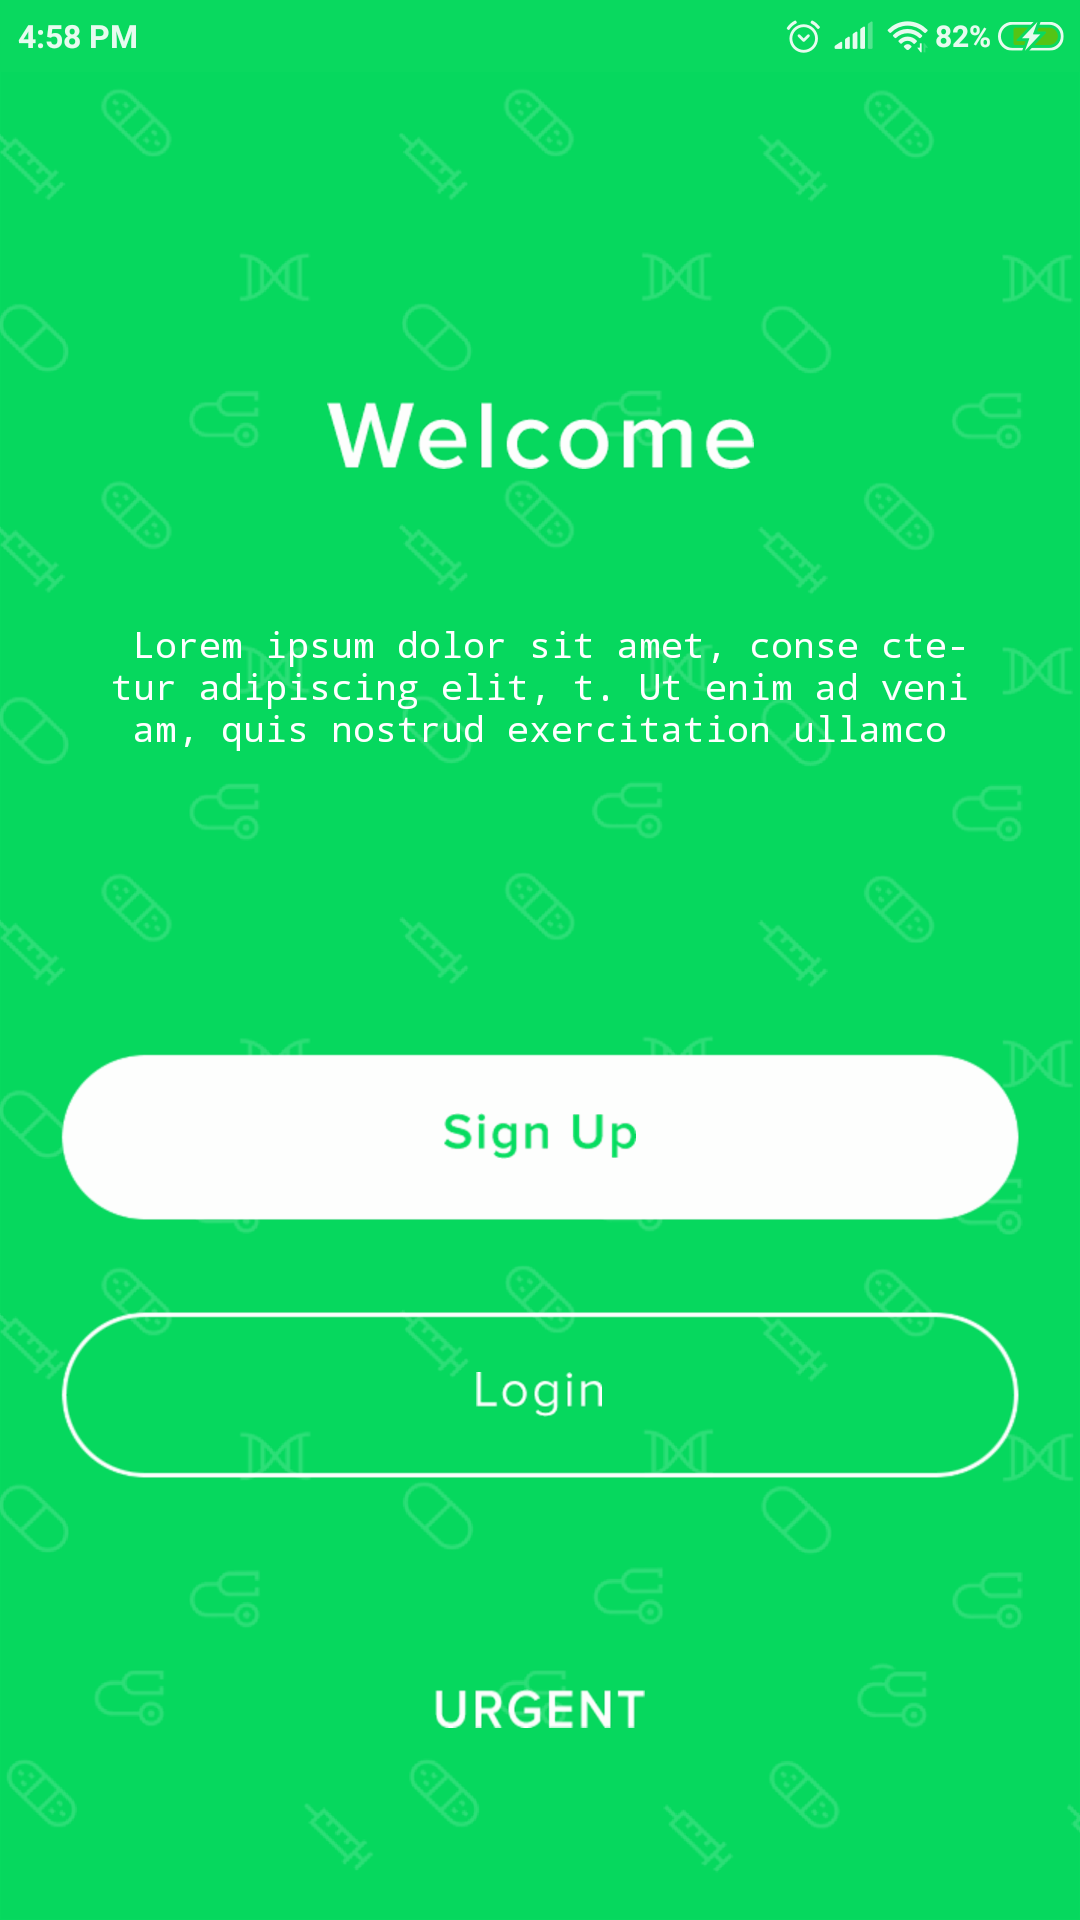
\includegraphics[scale=0.3]{img/Capture1.png}
\captionof{figure}{Main Activity}

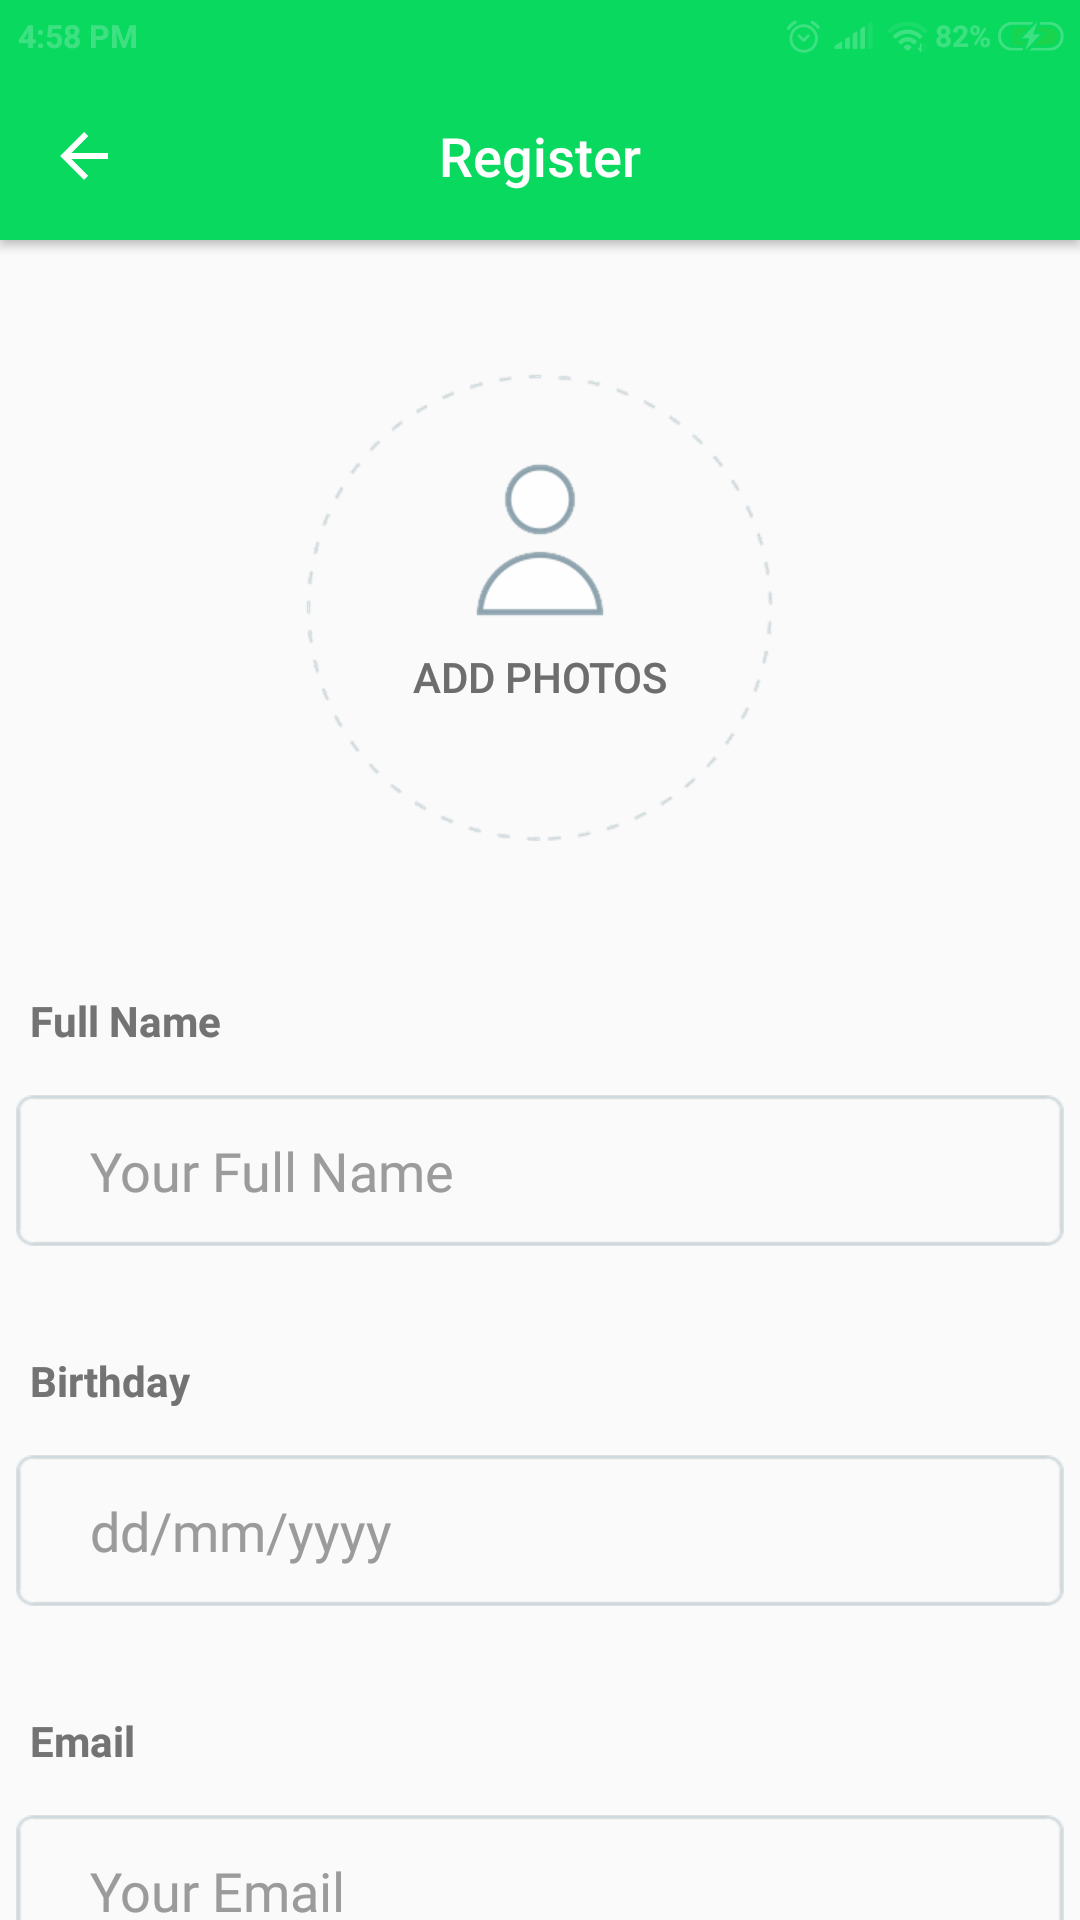
\includegraphics[scale=0.3]{img/Capture2.png}
\captionof{figure}{Sign up Activity}

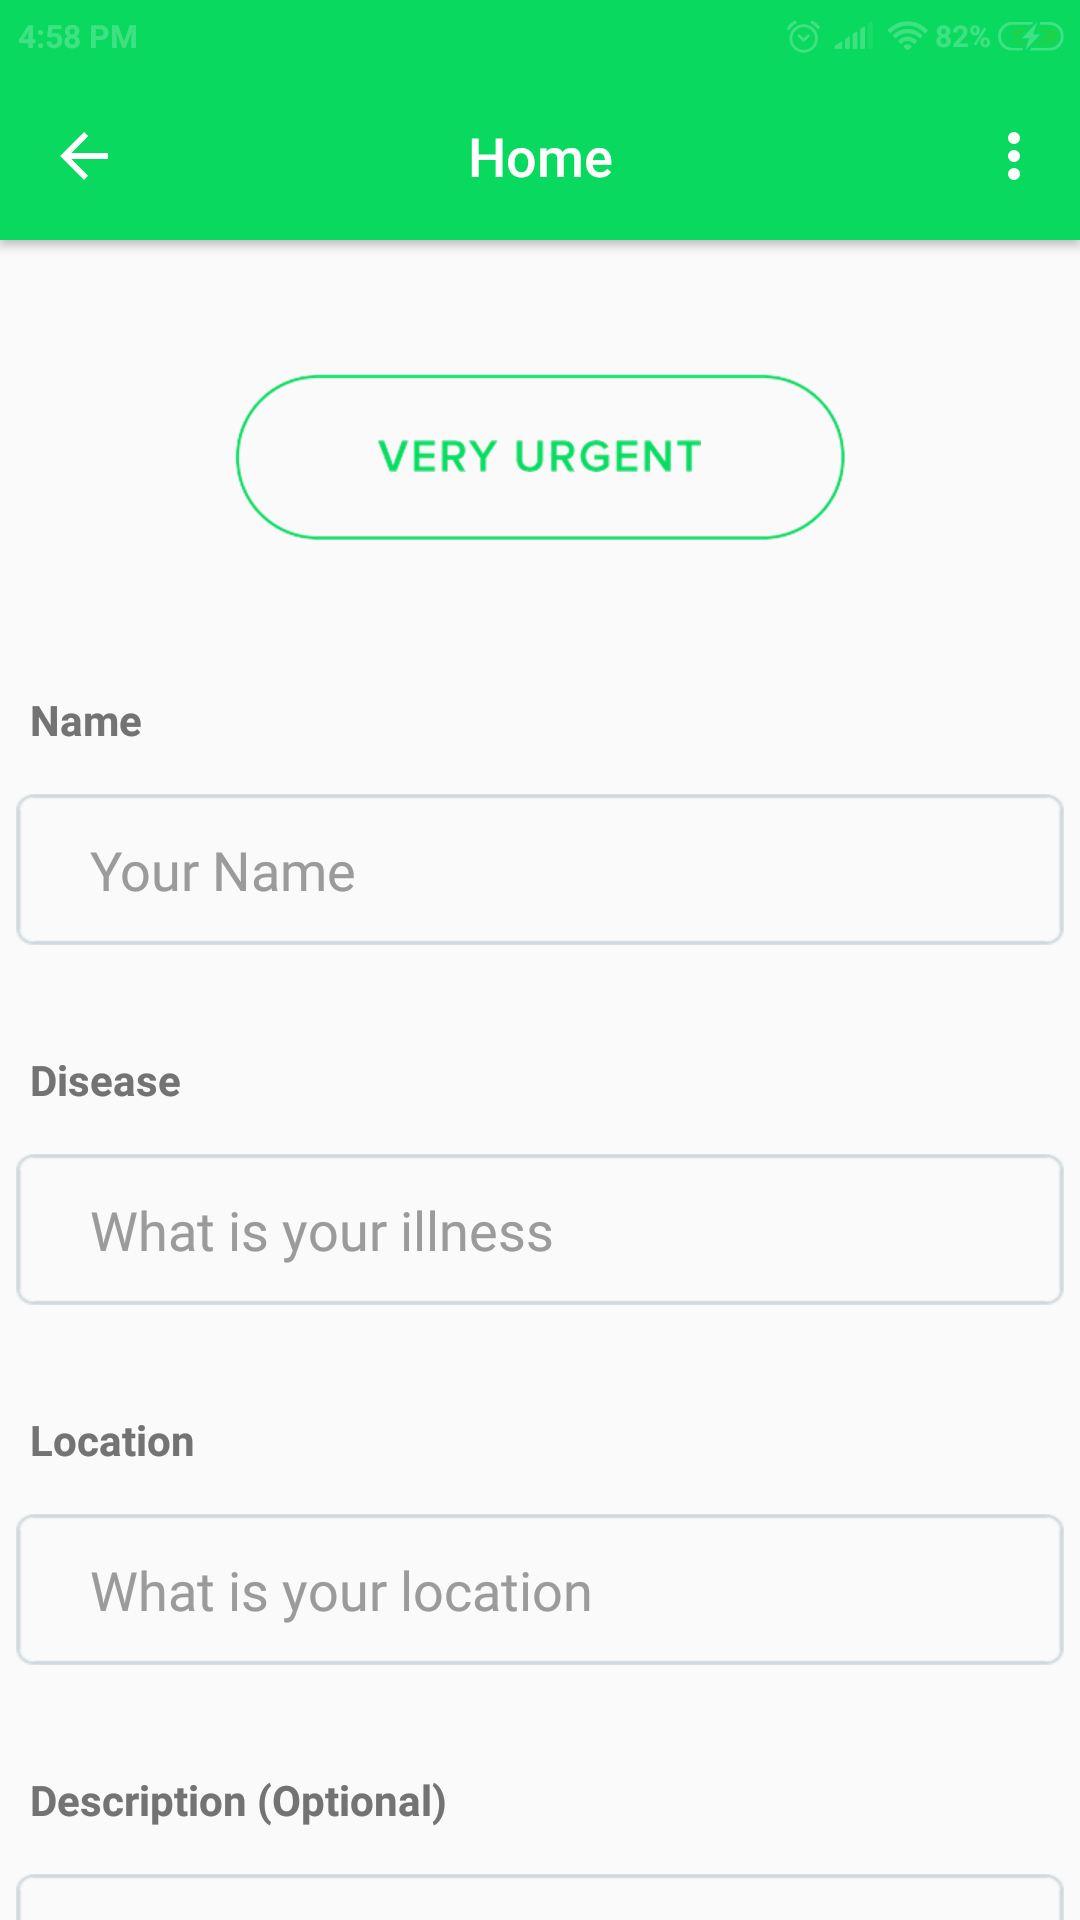
\includegraphics[scale=0.3]{img/Capture3.png}
\captionof{figure}{Home Activity}

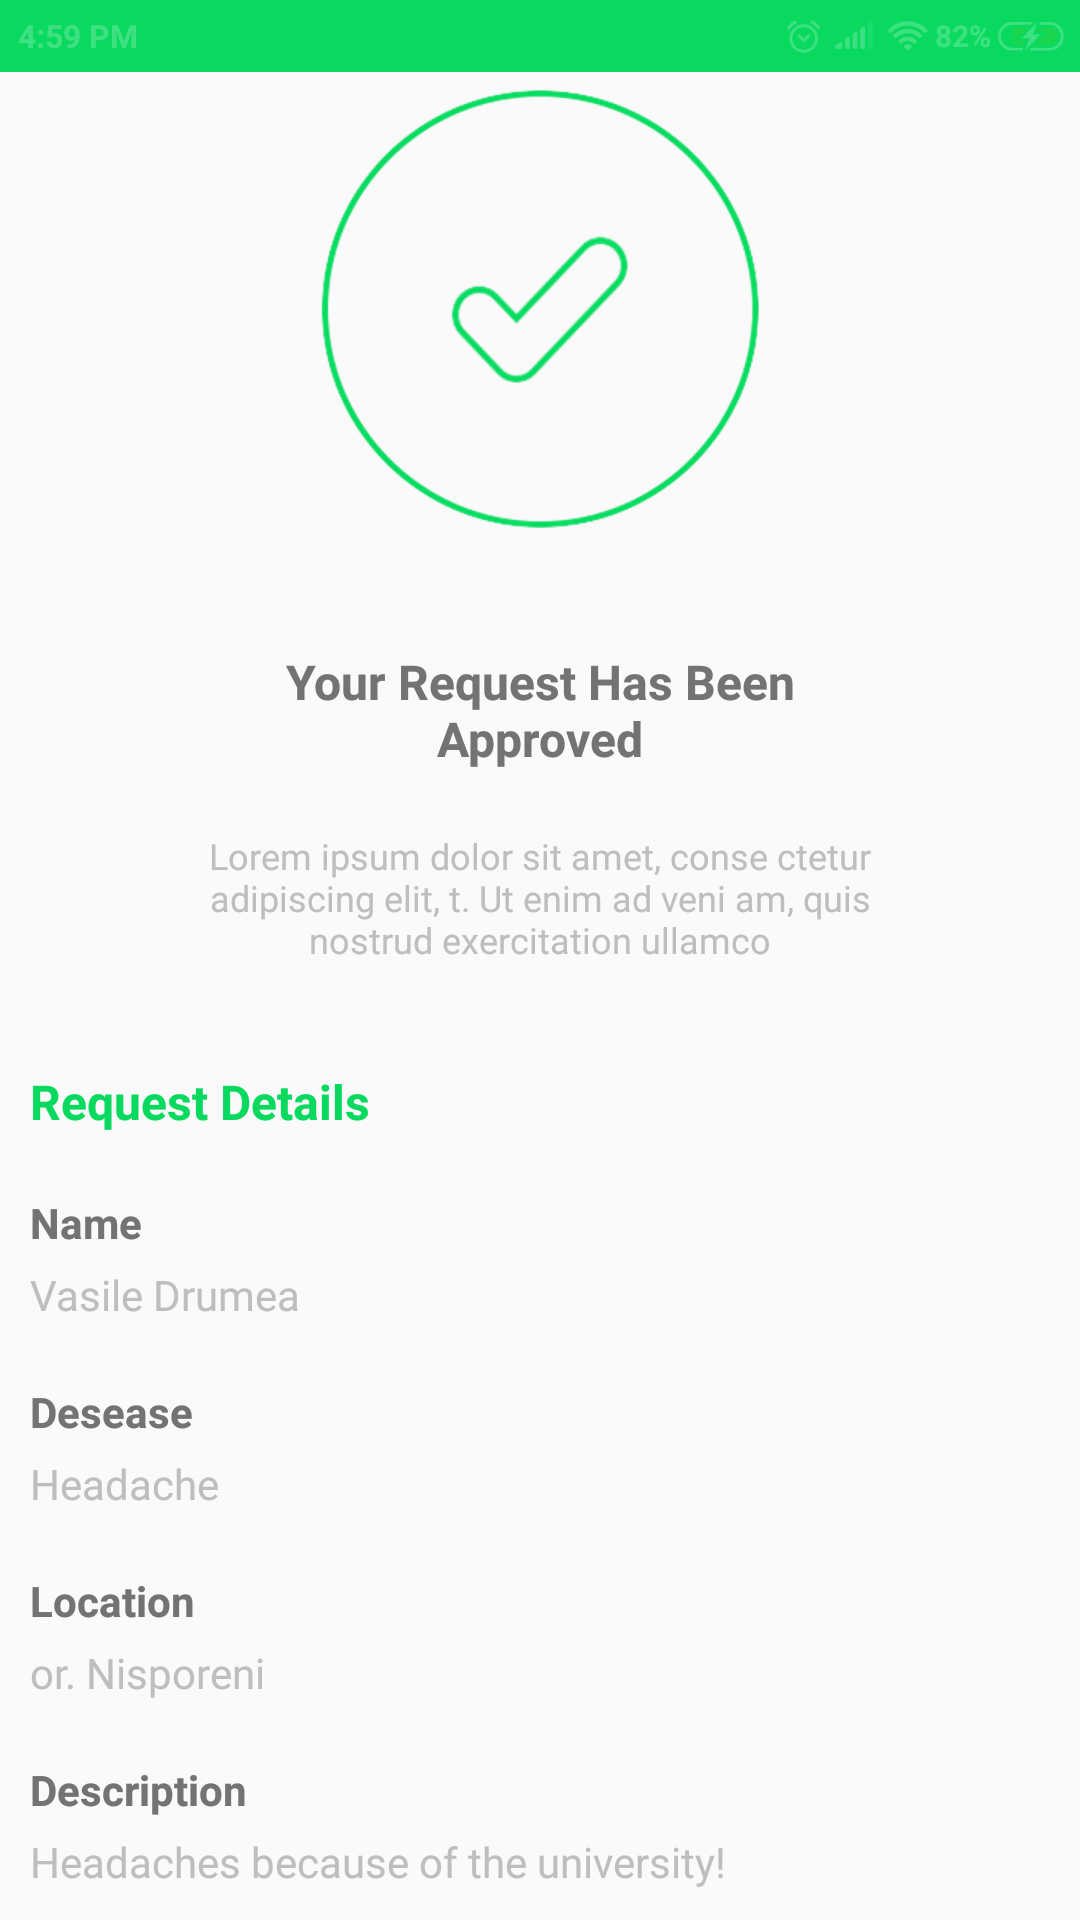
\includegraphics[scale=0.3]{img/Capture4.png}
\captionof{figure}{Request Activity}
\newpage

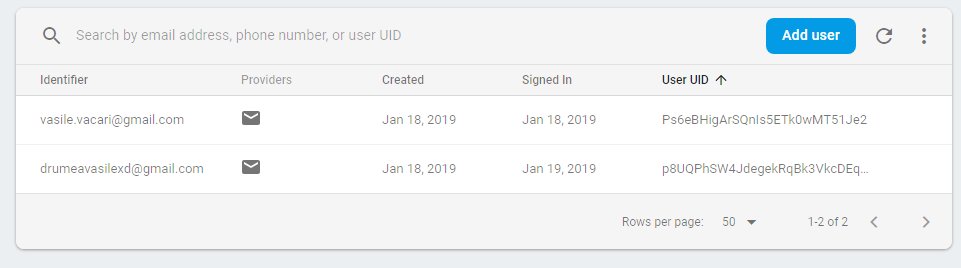
\includegraphics[scale=0.7]{img/Capture5.png}
\captionof{figure}{Firebase Console Authentication}

\end{center}
\clearpage